\documentclass{article}
\usepackage{graphicx} % Required for inserting images
\usepackage{xcolor}
\usepackage{algorithm}
\usepackage{algpseudocode}
\usepackage{listings}
\usepackage{tikz}
\usepackage{float}
\usepackage{amsmath, amssymb}
\usepackage{amsthm}

\lstset{language=C++}
\lstset{basicstyle=\ttfamily\small,
        keywordstyle=\color{blue},
        commentstyle=\color{green},
        stringstyle=\color{red},
        showstringspaces=false,
        numbers=left,
        numberstyle=\tiny,
        breaklines=true}
        
\title{Red-Black Trees}
\author{CS21B017 Chetan Moturi & CS21B033 Mallela Vidhyabhushan}
\date{April 2023}

\begin{document}
\maketitle

\section{Introduction}
A binary tree search tree of height can support basic operations like search, insert, and delete in logarithmic 
time, $O(\lg n)$, on average. However, the worst-case time complexity of these operations is $O(n)$. 
This is because the tree can degenerate into a linked list. To avoid this, we can use a self-balancing 
binary search tree. A self-balancing binary search tree is a binary search tree in which the height of the
tree is $O(\lg n)$. The height of a tree is the maximum number of edges from the root to a leaf. \\
One such self-balancing tree is called the Red-Black Tree. A red-black tree is a binary search tree in
which each node has an extra bit, and that bit is often interpreted as the color (red or black) of the
node. By constraining how the colors are used in any particular tree and how the tree is modified, we
can ensure that no path from the root to leaf is more than twice as long as any other path so that the
tree is approximately balanced. \\
\textbf{Fun Fact!}
The color "red" was chosen because it was the best-looking color produced by the color laser printer 
available to the authors while working at Xerox PARC.

\pagebreak

\section{Some Important Terminologies and Properties of Red-Black Trees}
The red-black tree is balanced by assigning a color to each node and ensuring that no path from the root to the leaf is twice as long as the other.\\
This ensures the tree is approximately balanced. The following code snippet shows the node structure of an RB Tree.

\begin{lstlisting}
enum Color {RED, BLACK, DOUBLE_BLACK};

struct Node
{
    int data;
    int color;
    Node *left, *right, *parent;

    explicit Node(int);
};
\end{lstlisting}

\begin{enumerate}
    \item \textbf{Color}: A red-black tree consists of one extra bit of storage compared to regular Binary search trees. A node can only be \textcolor{red}{RED} or \textcolor{black}{BLACK}.
    \item \textbf{Root Property}: The root is always BLACK.
    \item Every node is either \textcolor{black}{BLACK} or \textcolor{red}{RED}.
    \item \textbf{Sentinel Nodes}: If a child or parent of a node doesn't exist, we will assign them NIL. These are the leaves of the RB Tree, and other key-bearing nodes are called internal nodes.
    \item Every leaf is \textcolor{black}{BLACK}.
    \item If a node is \textcolor{red}{RED}, then both its children are \textcolor{black}{BLACK}
    \item \textbf{Black Height}: The number of black nodes on Every simple path from, but not including, node x to a leaf. It is denoted by bh(x).
    \item All nodes have an equal black height, i.e., an equal number of black nodes from the node to descendant leaves.
    \item The black height of a Red-Black Tree is the same as bh(root).
    \item The height of the red-black tree is at most $2\cdot\lg(N+1)$
    \item A Red-Black Tree of height h and number of nodes N, has $bh >$  $\frac{N}{2}$. 
\end{enumerate}

\pagebreak

\section{The RBTree class}
The Rb tree class with the required functions is given below,
\begin{lstlisting}
    class RBTree
{
    private:
        Node *root;
    protected:
        void rotateLeft(Node *&);
        void rotateRight(Node *&);
        void fixInsertRBTree(Node *&);
        void fixDeleteRBTree(Node *&);
        int getColor(Node *&);
        void setColor(Node *&, int);
        Node *minValueNode(Node *&);
        Node *maxValueNode(Node *&);
        Node* insertBST(Node *&, Node *&);
        Node* deleteBST(Node *&, int);
        int getBlackHeight(Node *);
    public:
        RBTree();
        void insertValue(int);
        void deleteValue(int);
        void merge(RBTree);
};
\end{lstlisting}
We will discuss these functions in detail now.

\section{Search in RB Tree}
Search in RB tree is as same as the search in a regular Binary search tree, but the search is a lot faster as the tree height is of $O(\lg n)$.
\\
The search algorithm Given a pointer to the root of the tree and a key k, Search
returns a pointer to a node with key k if one exists; otherwise, it returns NIL.
\begin{algorithm}
\caption{Red-Black Tree Search}
\begin{algorithmic}[1]
\Procedure{RbTreeSearch}{$T, x$}
    \If{$T = \text{null}$ or $x = T.\text{key}$}
        \State \Return $T$
    \ElsIf{$x < T.\text{key}$}
        \State \Return $\textsc{RbTreeSearch}(T.\text{left}, x)$
    \Else
        \State \Return $\textsc{RbTreeSearch}(T.\text{right}, x)$
    \EndIf
\EndProcedure
\end{algorithmic}
\end{algorithm}

\section{Insertion}
Inserting a node involves first searching through the tree to find its correct spot. Then the node is inserted there as a red node. Since it does not change the number of black nodes from any node to any of it’s leaves i.e the black height, the only issue we need to deal with is the violation of no red-red adjacent property.
\\
When inserting a new node into a Red-Black Tree, there are two possible cases that can arise depending on the color of the node's parent and uncle (the sibling of the node's parent).
\begin{enumerate}
    \item \textbf{CASE 1}: The uncle is \textcolor{red}{RED}.
    \item \textbf{CASE 2}: The uncle is BLACK.
        \begin{enumerate}
            \item \textbf{CASE 2.1}: Left-Left case.
            \item \textbf{CASE 2.2}: Left-Right case.
            \item \textbf{CASE 2.3}: Right-Left case.
            \item \textbf{CASE 2.4}: Right-Right case.
        \end{enumerate}
    \item Trivial cases: Parent is black.
\end{enumerate}
Let's discuss the cases in detail below,
\subsection{CASE 1: Uncle is Red}
In this case, we can simply recolor the parent, uncle, and grandparent nodes as black and red, respectively. We then repeat the same process for the grandparent node, which may violate the Red-Black Tree properties further up the tree. If the grandparent is the root, we simply recolor it as black to satisfy the root's black color property.\\
In the below tree, G is grandparent, U is uncle, P is parent and S is sibling of X.\\
\begin{center}
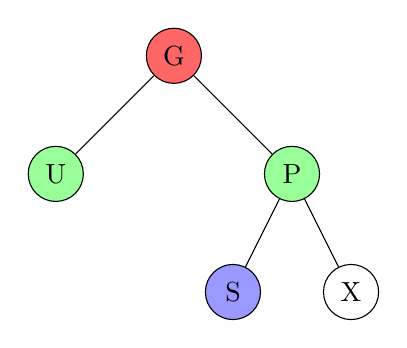
\begin{tikzpicture}[
  every node/.style={draw, circle, inner sep=2pt, minimum size=0.7cm},
  level/.style={sibling distance=3cm/#1, level distance=1.5cm},
  blue/.style={fill=blue!40},
  green/.style={fill=green!40},
  red/.style={fill=red!60}
]
\node[red] {G}
  child[blue] {node[green] {U}
  }
  child {node[green] {P}
    child {node[blue] {S}}
    child {node {X}}
  };
\end{tikzpicture}
\end{center}
\pagebreak
Initially the tree is as follows, with X being the node that is inserted,
\begin{center}
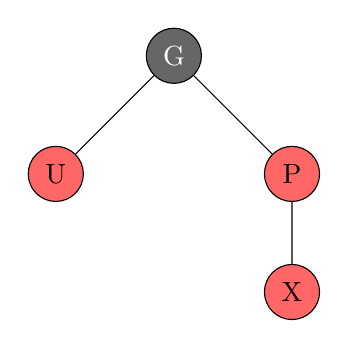
\begin{tikzpicture}[
  every node/.style={draw, circle, inner sep=2pt, minimum size=0.7cm},
  level/.style={sibling distance=3cm/#1, level distance=1.5cm},
  black/.style={fill=black!60, text=white},
  red/.style={fill=red!60}
]
\node[black] {G}
  child {node[red] {U}
  }
  child {node[red] {P}
    child {node[red] {X}}
  };
\end{tikzpicture}
\end{center}
We know that the inserted node's grandparent will be black, so all we need to do is switch the coloring of the inserted node's grandparent with the coloring of the inserted node's parent and its parent's sibling. This case might need to continue to be fixed up through the root of the tree, though, because the inserted node's grandparent may have a parent who is red.
\\Hence the final tree is,
\begin{center}
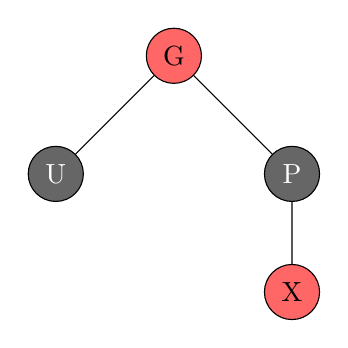
\begin{tikzpicture}[
  every node/.style={draw, circle, inner sep=2pt, minimum size=0.7cm},
  level/.style={sibling distance=3cm/#1, level distance=1.5cm},
  black/.style={fill=black!60, text=white},
  red/.style={fill=red!60}
]
\node[red] {G}
  child {node[black] {U}
  }
  child {node[black] {P}
    child {node[red] {X}}
  };
\end{tikzpicture}
\end{center}

\subsection{CASE 2: Uncle is Black}
As discussed before there are four sub-cases in this scenario. Let's discuss their respective solutions.
\subsubsection{Left-Left Case}
If the node's parent is the left child of the grandparent and the inserted node is the left child of the parent.\\
\textbf{Solution} : Right rotate Grandfather(parent’s parent) and swap the colors of grandparent and parent of the node.\\
Let us look at an example, once again we are inserting node X,
\begin{center}
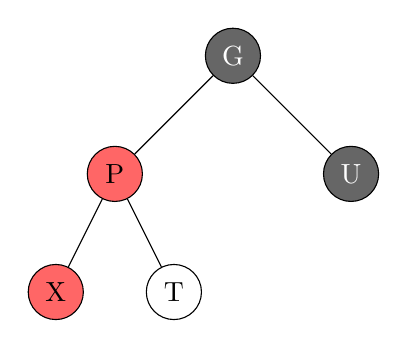
\begin{tikzpicture}[
  every node/.style={draw, circle, inner sep=2pt, minimum size=0.7cm},
  level/.style={sibling distance=3cm/#1, level distance=1.5cm},
  black/.style={fill=black!60, text=white},
  red/.style={fill=red!60}
]
\node[black] {G}
  child {node[red] {P}
    child {node[red] {X}}
    child {node {T}}
  }
  child {node[black] {U}
  };
\end{tikzpicture}
\end{center}
After Right rotation of Grandfather, swap colors of grandfather and parent. The final tree will look like,
\begin{center}
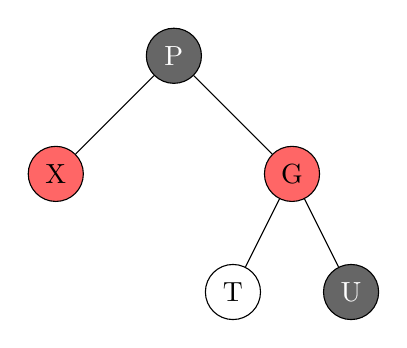
\begin{tikzpicture}[
  every node/.style={draw, circle, inner sep=2pt, minimum size=0.7cm},
  level/.style={sibling distance=3cm/#1, level distance=1.5cm},
  black/.style={fill=black!60, text=white},
  red/.style={fill=red!60}
]
\node[black] {P}
  child {node[red] {X}
  }
  child {node[red] {G}
    child {node {T}}
    child {node[black] {U}}
  };
\end{tikzpicture}
\end{center}

\subsubsection{Left-Right Case}
the node's parent is the left child of the grandparent and the inserted node is the right child of the parent.\\
\textbf{Solution}: Left rotate the parent and then apply Left-left rotate on the parent. Swap the colors of the inserted node and the grandparent.
Let's look at an example,
\begin{center}
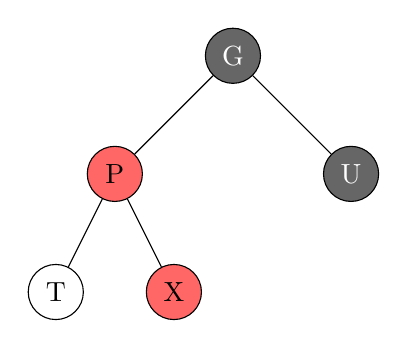
\begin{tikzpicture}[
  every node/.style={draw, circle, inner sep=2pt, minimum size=0.7cm},
  level/.style={sibling distance=3cm/#1, level distance=1.5cm},
  black/.style={fill=black!60, text=white},
  red/.style={fill=red!60}
]
\node[black] {G}
  child {node[red] {P}
    child {node {T}}
    child {node[red] {X}}
  }
  child {node[black] {U}
  };
\end{tikzpicture}
\end{center}
After Left rotate parent, then apply case 5.2.1, we have the final tree,
\begin{center}
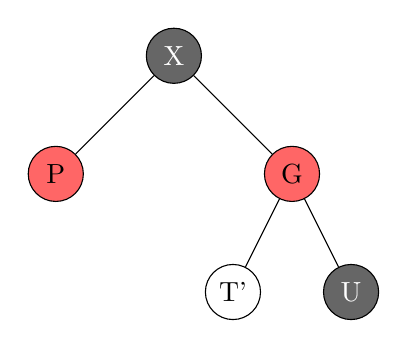
\begin{tikzpicture}[
  every node/.style={draw, circle, inner sep=2pt, minimum size=0.7cm},
  level/.style={sibling distance=3cm/#1, level distance=1.5cm},
  black/.style={fill=black!60, text=white},
  red/.style={fill=red!60}
]
\node[black] {X}
  child {node[red] {P}
  }
  child {node[red] {G}
    child {node {T'}}
    child {node[black] {U}}
  };
\end{tikzpicture}
\end{center}

\subsubsection{Right-Right Case}
The node’s parent is the right child of the grandparent and the inserted node is the right child of the parent.\\
\textbf{Solution}: Left rotate Grandfather(parent’s parent) and swap the colors of grandparent and parent of the node.
Let's look at an example,
\begin{center}
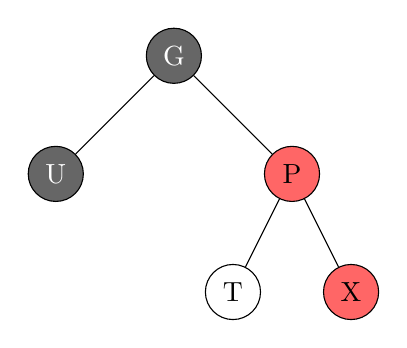
\begin{tikzpicture}[
  every node/.style={draw, circle, inner sep=2pt, minimum size=0.7cm},
  level/.style={sibling distance=3cm/#1, level distance=1.5cm},
  black/.style={fill=black!60, text=white},
  red/.style={fill=red!60}
]
\node[black] {G}
  child {node[black] {U}
  }
  child {node[red] {P}
    child {node {T}}
    child {node[red] {X}}
  };
\end{tikzpicture}
\end{center}
After fixing up the tree by the above solution we have the final tree as,

\begin{center}
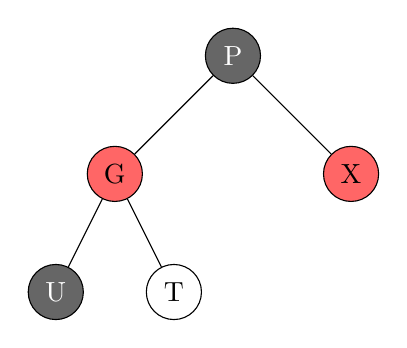
\begin{tikzpicture}[
  every node/.style={draw, circle, inner sep=2pt, minimum size=0.7cm},
  level/.style={sibling distance=3cm/#1, level distance=1.5cm},
  black/.style={fill=black!60, text=white},
  red/.style={fill=red!60}
]
\node[black] {P}
  child {node[red] {G}
    child{node[black] {U}}
    child{node {T}}
  }
  child {node[red] {X}
  };
\end{tikzpicture}
\end{center}

\subsubsection{Right-Left Case}
the node's parent is the right child of the grandparent and the inserted node is the left child of the parent.
\textbf{Solution}: Right rotate the parent of the inserted node and then apply the right-right rotate on the parent node. Swap the colors of the inserted node and the grandparent.
Let's look at an example,

\begin{center}
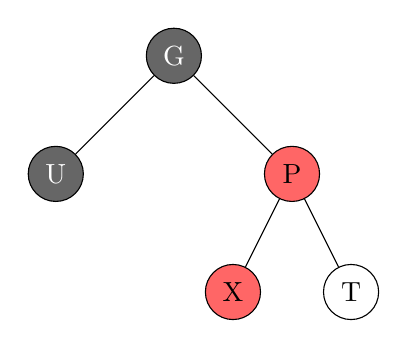
\begin{tikzpicture}[
  every node/.style={draw, circle, inner sep=2pt, minimum size=0.7cm},
  level/.style={sibling distance=3cm/#1, level distance=1.5cm},
  black/.style={fill=black!60, text=white},
  red/.style={fill=red!60}
]
\node[black] {G}
  child {node[black] {U}
  }
  child {node[red] {P}
    child{node[red] {X}}
    child{node {T}}
  };
\end{tikzpicture}
\end{center}
After fixing the tree up we have the resulting tree,
\begin{center}
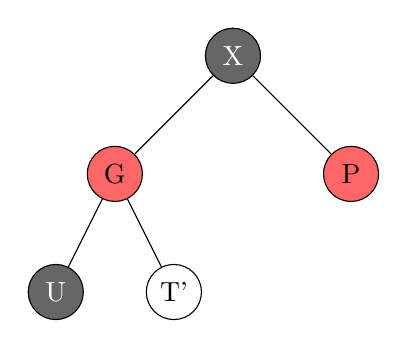
\begin{tikzpicture}[
  every node/.style={draw, circle, inner sep=2pt, minimum size=0.7cm},
  level/.style={sibling distance=3cm/#1, level distance=1.5cm},
  black/.style={fill=black!60, text=white},
  red/.style={fill=red!60}
]
\node[black] {X}
  child {node[red] {G}
    child {node[black] {U}}
    child {node {T'}}
  }
  child {node[red] {P}
  };
\end{tikzpicture}
\end{center}
\pagebreak
\subsection{Pseudo code for Insertion and Insertion Fixup}

\begin{algorithm}
\caption{RB-Tree Insertion}
\begin{algorithmic}[1]
\Procedure{RB-INSERT}{$T,z$}
  \State $y \gets \text{NIL}$
  \State $x \gets T.root$
  \While{$x \neq \text{NIL}$}
    \State $y \gets x$
    \If{$z.key < x.key$}
      \State $x \gets x.left$
    \Else
      \State $x \gets x.right$
    \EndIf
  \EndWhile
  \State $z.p \gets y$
  \If{$y = \text{NIL}$}
    \State $T.root \gets z$
  \ElsIf{$z.key < y.key$}
    \State $y.left \gets z$
  \Else
    \State $y.right \gets z$
  \EndIf
  \State $z.left \gets \text{NIL}$
  \State $z.right \gets \text{NIL}$
  \State $z.color \gets \text{RED}$
  \State \Call{RB-INSERT-FIXUP}{$T,z$}
\EndProcedure
\end{algorithmic}
\end{algorithm}

\begin{algorithm}
    \caption{RB-Tree Insertion Fixup}
    \begin{algorithmic}
        \Procedure{RB-INSERT-FIXUP}{$T,z$}
  \While{$z.p.color = \text{RED}$}
    \If{$z.p = z.p.p.left$}
      \State $y \gets z.p.p.right$
      \If{$y.color = \text{RED}$}
        \State $z.p.color \gets \text{BLACK}$
        \State $y.color \gets \text{BLACK}$
        \State $z.p.p.color \gets \text{RED}$
        \State $z \gets z.p.p$
      \Else
        \If{$z = z.p.right$}
          \State $z \gets z.p$
          \State \Call{LEFT-ROTATE}{$T,z$}
        \EndIf
        \State $z.p.color \gets \text{BLACK}$
        \State $z.p.p.color \gets \text{RED}$
        \State \Call{RIGHT-ROTATE}{$T,z.p.p$}
      \EndIf
    \Else
      \State $y \gets z.p.p.left$
      \If{$y.color = \text{RED}$}
        \State $z.p.color \gets \text{BLACK}$
        \State $y.color \gets \text{BLACK}$
        \State $z.p.p.color \gets \text{RED}$
        \State $z \gets z.p.p$
      \Else
        \If{$z = z.p.left$}
          \State $z \gets z.p$
          \State \Call{RIGHT-ROTATE}{$T,z$}
        \EndIf
        \State $z.p.color \gets \text{BLACK}$
        \State $z.p.p.color \gets \text{RED}$
        \State \Call{LEFT-ROTATE}{$T,z.p.p$}
      \EndIf
    \EndIf
  \EndWhile
  \State $T.root.color \gets \text{BLACK}$
\EndProcedure

    \end{algorithmic}
\end{algorithm}
\pagebreak
\section{Deletion}
Like other basic operations on the RB Tree deletion takes time $O(\lg n)$. Deleting a node from a RB Tree is more complicated than insertion. When a node is deleted it can either have no children, one child or two children.In delete, the main violated property is, change of black height in sub trees as deletion of a black node may cause reduced black height in one root to leaf path.\\
To understand deletion, the notion of \textbf{double black} is used.  When a black node is deleted and replaced by a black child, the child is marked as \textbf{double black}. The main task now becomes to convert this \textbf{double black} to single black. \\
To delete a node from a Red Black Tree follow the steps as given below,
\begin{enumerate}
    \item \textbf{Perform standard BST delete}: When we perform standard delete operation in BST, we always end up deleting a node which is an either leaf or has only one child (For an internal node, we copy the successor and then recursively call delete for successor, successor is always a leaf node or a node with one child). So we only need to handle cases where a node is leaf or has one child. Let v be the node to be deleted and u be the child that replaces v (Note that u is NULL when v is a leaf and color of NULL is considered as Black).
    \item \textbf{Simple Case: If either u or v is red}
    \item \textbf{Complex Case: If Both u and v are Black}.
    \begin{enumerate}
        \item colour u as double black.
        \item \textbf{NOTE!} If v is a leaf, then u is NULL, and the colour of NULL is considered black.
        \item For a sibling node s of current node u that is double black but not the root,
        \begin{enumerate}
            \item \textbf{case 1}: If sibling node s is black and at least one of its children is red. This will again contain the sub cases of RR, RL, LR and LL. 
            \item \textbf{case 2}: If the sibling s is black and both of its children are black.
            \item \textbf{case 3}: If sibling s is red, perform a rotation to move the old sibling node up,recolor the old sibling and parent. The new sibling is always black. This converts the tree to the black sibling case (by rotation) and leads to previous cases. This case is divided into two sub cases; left and right cases.
        \end{enumerate}
    \end{enumerate}
    \item If u is the root, make it single black.
\end{enumerate}
Let's discuss the cases possible in detail along with their respective examples,
\subsection{Simple Case: Either u or v is red}
Here as mentioned before, v is the node to be deleted and u is the child which replaced v. We mark the replaced child as black (deletion causes no change in black height). Note that as v is the parent of u, and two consecutive reds are not allowed in the red-black tree, both u and v cannot be red.
Let's look at the example below,

\begin{center}
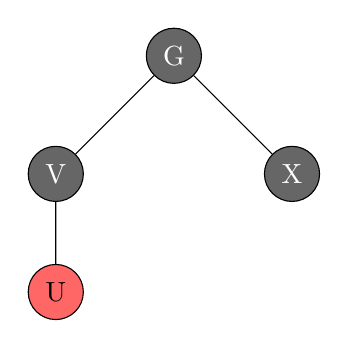
\begin{tikzpicture}[
  every node/.style={draw, circle, inner sep=2pt, minimum size=0.7cm},
  level/.style={sibling distance=3cm/#1, level distance=1.5cm},
  black/.style={fill=black!60, text=white},
  red/.style={fill=red!60}
]
\node[black] {G}
  child {node[black] {V}
    child {node[red] {U}}
  }
  child {node[black] {X}
  };
\end{tikzpicture}
\end{center}
Since we are deleting V, we replace it with U and make U black to preserve the black height. So the final tree looks like,
\begin{center}
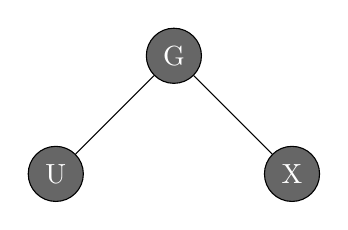
\begin{tikzpicture}[
  every node/.style={draw, circle, inner sep=2pt, minimum size=0.7cm},
  level/.style={sibling distance=3cm/#1, level distance=1.5cm},
  black/.style={fill=black!60, text=white},
  red/.style={fill=red!60}
]
\node[black] {G}
  child {node[black] {U}
  }
  child {node[black] {X}
  };
\end{tikzpicture}
\end{center}

\subsection{Complex Case: Both u and v are black}
color the node u as double black. Now, the task is to convert the double black into single black. If v is leaf then u is NIL so it is a black node. Hence deletion of black leaf causes double black.

\begin{center}
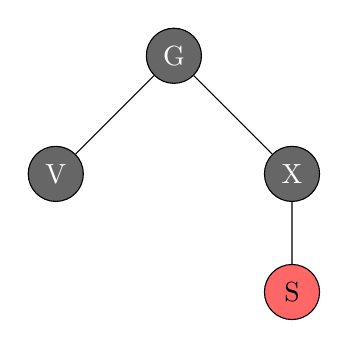
\begin{tikzpicture}[
  every node/.style={draw, circle, inner sep=2pt, minimum size=0.7cm},
  level/.style={sibling distance=3cm/#1, level distance=1.5cm},
  black/.style={fill=black!60, text=white},
  red/.style={fill=red!60}
]
\node[black] {G}
  child {node[black] {V}
  }
  child {node[black] {X}
    child{node[red] {S}}
  };
\end{tikzpicture}
\end{center}
After deleting V we get the tree,
\begin{center}
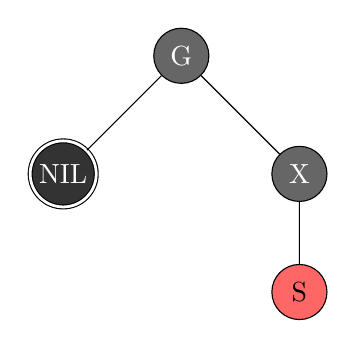
\begin{tikzpicture}[
  every node/.style={draw, circle, inner sep=2pt, minimum size=0.7cm},
  level/.style={sibling distance=3cm/#1, level distance=1.5cm},
  black/.style={fill=black!60, text=white},
  red/.style={fill=red!60},
  doubleblack/.style={fill=black!80, text=white, double=white, double distance=1pt}
]
\node[black] {G}
  child {node[doubleblack] {NIL}
  }
  child {node[black] {X}
    child{node[red] {S}}
  };
\end{tikzpicture}
\end{center}
In the above tree we see u becomes a double black NIL node.\\
Now we'll see the cases for a sibling node s for a double black node u which is not the root,
\subsubsection{If sibling node s is black and at least one of its children is red}
We need to perform rotations to re-balance the tree, as such this consists of four different sub cases depending on the relative position of s and r, the red child of s.
\paragraph{Right-Right case:}
In this case, S is right child of it's parent and R is right child of S.\\
\textbf{Conditions}:
\begin{enumerate}
    \item Double Black's sibling is black.
    \item Double Black's sibling's far child is \textcolor{red}{red}
\end{enumerate}
\textbf{Solution}:
\begin{enumerate}
    \item Swap color of DB's parent with DB's sibling's color.
    \item Perform rotation at DB's parent in direction of DB.
    \item Remove DB sign and make the node normal black node.
    \item Change colour of DB's sibling's far red child to black.
\end{enumerate}

Let us look at an example for better understanding, The tree at its double black stage is given below,
\begin{center}
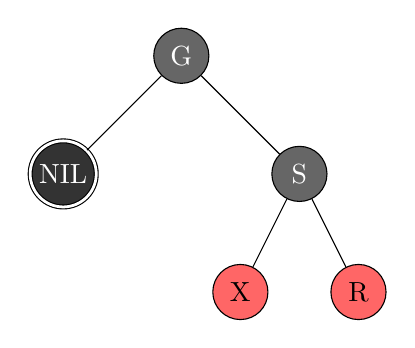
\begin{tikzpicture}[
  every node/.style={draw, circle, inner sep=2pt, minimum size=0.7cm},
  level/.style={sibling distance=3cm/#1, level distance=1.5cm},
  black/.style={fill=black!60, text=white},
  red/.style={fill=red!60},
  doubleblack/.style={fill=black!80, text=white, double=white, double distance=1pt}
]
\node[black] {G}
  child {node[doubleblack] {NIL}
  }
  child {node[black] {S}
    child{node[red] {X}}
    child{node[red] {R}}
  };
\end{tikzpicture}
\end{center}
After performing the above steps we get the tree,
\begin{center}
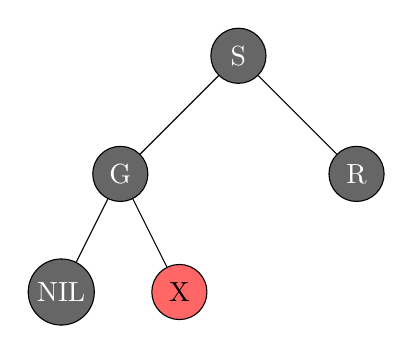
\begin{tikzpicture}[
  every node/.style={draw, circle, inner sep=2pt, minimum size=0.7cm},
  level/.style={sibling distance=3cm/#1, level distance=1.5cm},
  black/.style={fill=black!60, text=white},
  red/.style={fill=red!60},
  doubleblack/.style={fill=black!80, text=white, double=white, double distance=1pt}
]
\node[black] {S}
  child {node[black] {G}
    child{node[black] {NIL}}
    child{node[red] {X}}
  }
  child {node[black] {R}
  };
\end{tikzpicture}
\end{center}

\paragraph{Right-Left Case:}
In this case S is the right child of its parent and R is the red left child of S.\\
\textbf{Conditions}:
\begin{enumerate}
    \item Double Black's sibling is black.
    \item Double Black's sibling's far child is black.
    \item DB's sibling's child which is near is \textcolor{red}{red}.
\end{enumerate}
\textbf{Solution}:
\begin{enumerate}
    \item Swap color of sibling with sibling's \textcolor{red}{red} child.
    \item Perform rotation at sibling node in direction opposite of DB.
    \item apply the previous case.
\end{enumerate}
Let us look at the example below, V has been deleted and U is double black, T is any sub-tree/node.
\begin{center}
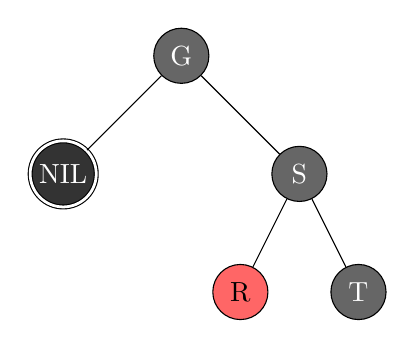
\begin{tikzpicture}[
  every node/.style={draw, circle, inner sep=2pt, minimum size=0.7cm},
  level/.style={sibling distance=3cm/#1, level distance=1.5cm},
  black/.style={fill=black!60, text=white},
  red/.style={fill=red!60},
  doubleblack/.style={fill=black!80, text=white, double=white, double distance=1pt}
]
\node[black] {G}
  child {node[doubleblack] {NIL}
  }
  child {node[black] {S}
    child{node[red] {R}}
    child{node[black] {T}}
  };
\end{tikzpicture}
\end{center}
After performing the first two steps we get the tree,
\begin{center}
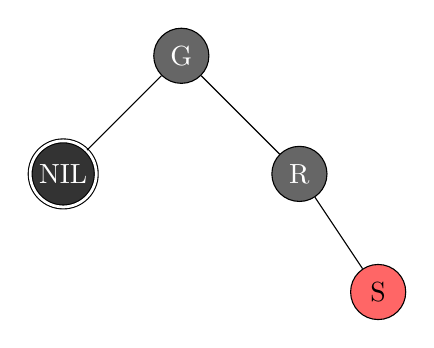
\begin{tikzpicture}[
  every node/.style={draw, circle, inner sep=2pt, minimum size=0.7cm},
  level/.style={sibling distance=3cm/#1, level distance=1.5cm},
  black/.style={fill=black!60, text=white},
  red/.style={fill=red!60},
  doubleblack/.style={fill=black!80, text=white, double=white, double distance=1pt}
]
\node[black] {G}
  child {node[doubleblack] {NIL}
  }
  child {node[black] {R}
    child{node[xshift=1cm][red] {S}}
  };
\end{tikzpicture}
\end{center}
Here, T is a sentinel node (or any sub-tree).\\
Now, we can apply the right-right case and re balance the tree.
\begin{center}
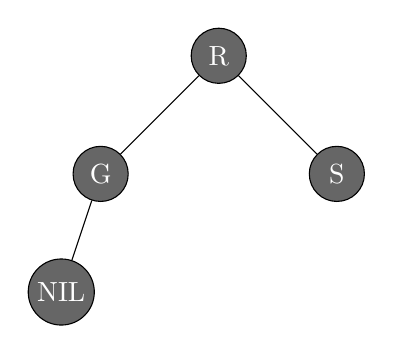
\begin{tikzpicture}[
  every node/.style={draw, circle, inner sep=2pt, minimum size=0.7cm},
  level/.style={sibling distance=3cm/#1, level distance=1.5cm},
  black/.style={fill=black!60, text=white},
  red/.style={fill=red!60},
  doubleblack/.style={fill=black!80, text=white, double=white, double distance=1pt}
]
\node[black] {R}
  child {node[black] {G}
    child{node[xshift=-0.5cm][black] {NIL}}
  }
  child {node[black] {S}
  };
\end{tikzpicture}
\end{center}

\paragraph{Left-Left Case:}
where s is left child of its parent and r is left child of s; it is mirror case of the right-right case.
\paragraph{Left-Right Case:}
where s is left child of its parent and r is right child of s; it is mirror case of the left-right case.

\subsubsection{If the sibling S is black and both of its children are black}
The solution to the above case is as follows,
\begin{enumerate}
    \item Remove the DB(if NIL-DB remove the node, for other nodes, remove the DB sign.
    \item Make DB's sibling \textcolor{red}{red}.
    \item If DB's parent is black make it DB, else make it black.
\end{enumerate}
This will become clear with the following example, the initial tree is given below and we will remove,
\begin{center}
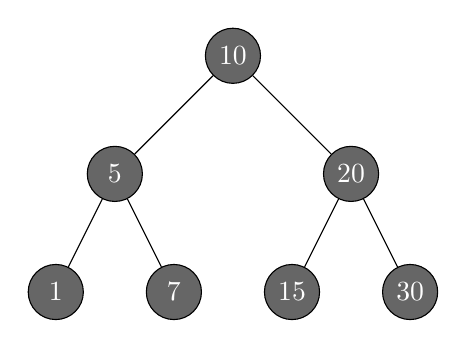
\begin{tikzpicture}[
  every node/.style={draw, circle, inner sep=2pt, minimum size=0.7cm},
  level/.style={sibling distance=3cm/#1, level distance=1.5cm},
  black/.style={fill=black!60, text=white},
  red/.style={fill=red!60},
  doubleblack/.style={fill=black!80, text=white, double=white, double distance=1pt}
]
\node[black] {10}
  child {node[black] {5}
    child{node[black] {1}}
    child{node[black] {7}}
  }
  child {node[black] {20}
    child{node[black] {15}}
    child{node[black] {30}}
  };
\end{tikzpicture}
\end{center}
After deleting 15 we get, 
\begin{center}
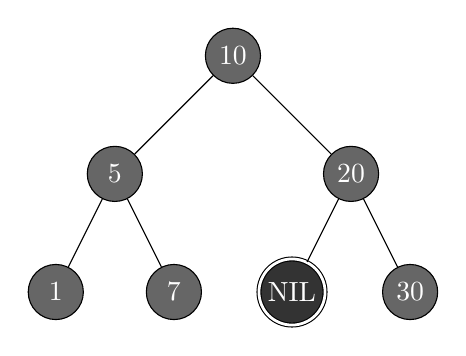
\begin{tikzpicture}[
  every node/.style={draw, circle, inner sep=2pt, minimum size=0.7cm},
  level/.style={sibling distance=3cm/#1, level distance=1.5cm},
  black/.style={fill=black!60, text=white},
  red/.style={fill=red!60},
  doubleblack/.style={fill=black!80, text=white, double=white, double distance=1pt}
]
\node[black] {10}
  child {node[black] {5}
    child{node[black] {1}}
    child{node[black] {7}}
  }
  child {node[black] {20}
    child{node[doubleblack] {NIL}}
    child{node[black] {30}}
  };
\end{tikzpicture}
\end{center}
After performing steps 2 \& 3 we get,
\begin{center}
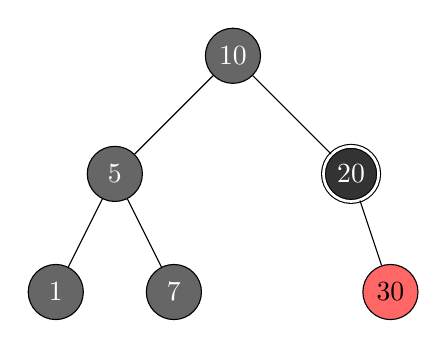
\begin{tikzpicture}[
  every node/.style={draw, circle, inner sep=2pt, minimum size=0.7cm},
  level/.style={sibling distance=3cm/#1, level distance=1.5cm},
  black/.style={fill=black!60, text=white},
  red/.style={fill=red!60},
  doubleblack/.style={fill=black!80, text=white, double=white, double distance=1pt}
]
\node[black] {10}
  child {node[black] {5}
    child{node[black] {1}} 
    child{node[black] {7}}
  }
  child {node[doubleblack] {20}
    child{node[xshift=0.5cm][red] {30}}
  };
\end{tikzpicture}
\end{center}
Repeat this again for the double black-20, we get,
\begin{center}
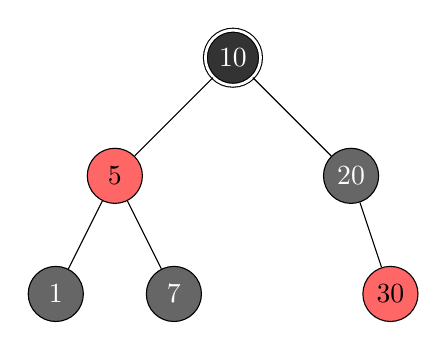
\begin{tikzpicture}[
  every node/.style={draw, circle, inner sep=2pt, minimum size=0.7cm},
  level/.style={sibling distance=3cm/#1, level distance=1.5cm},
  black/.style={fill=black!60, text=white},
  red/.style={fill=red!60},
  doubleblack/.style={fill=black!80, text=white, double=white, double distance=1pt}
]
\node[doubleblack] {10}
  child {node[red] {5}
    child{node[black] {1}} 
    child{node[black] {7}}
  }
  child {node[black] {20}
    child{node[xshift=0.5cm][red] {30}}
  };
\end{tikzpicture}
\end{center}
Since DB is the root we can demote it to black, giving us the final tree as,
\begin{center}
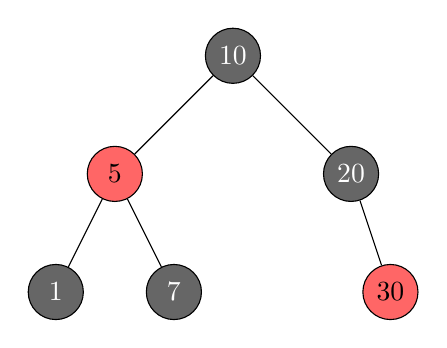
\begin{tikzpicture}[
  every node/.style={draw, circle, inner sep=2pt, minimum size=0.7cm},
  level/.style={sibling distance=3cm/#1, level distance=1.5cm},
  black/.style={fill=black!60, text=white},
  red/.style={fill=red!60},
  doubleblack/.style={fill=black!80, text=white, double=white, double distance=1pt}
]
\node[black] {10}
  child {node[red] {5}
    child{node[black] {1}} 
    child{node[black] {7}}
  }
  child {node[black] {20}
    child{node[xshift=0.5cm][red] {30}}
  };
\end{tikzpicture}
\end{center}

\subsubsection{If sibling S is \textcolor{red}{red}}
The solution to the above case is as follows,
\begin{enumerate}
    \item swap DB'S parent's and S's colors.
    \item perform rotation at parent node in direction of DB.
    \item check which case can be applied to the new tree and re-balance the tree.
\end{enumerate}
Let's see the example below,
\begin{center}
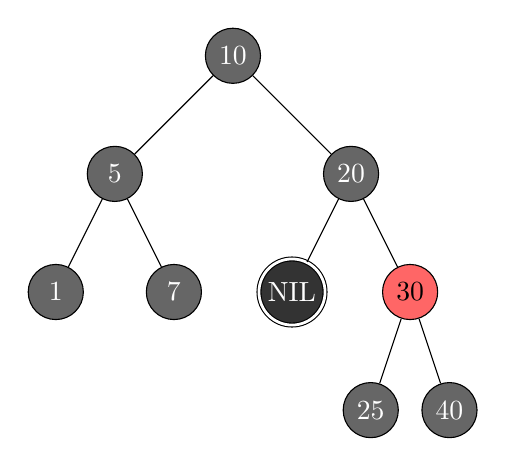
\begin{tikzpicture}[
  every node/.style={draw, circle, inner sep=2pt, minimum size=0.7cm},
  level/.style={sibling distance=3cm/#1, level distance=1.5cm},
  black/.style={fill=black!60, text=white},
  red/.style={fill=red!60},
  doubleblack/.style={fill=black!80, text=white, double=white, double distance=1pt}
]
\node[black] {10}
  child {node[black] {5}
    child{node[black] {1}} 
    child{node[black] {7}}
  }
  child {node[black] {20}
    child{node[doubleblack] {NIL}}
    child{node[red] {30}
        child{node[black]{25}}
        child{node[black]{40}}
    }
  };
\end{tikzpicture}
\end{center}
After fixing the tree by the above rules we get,
\begin{center}
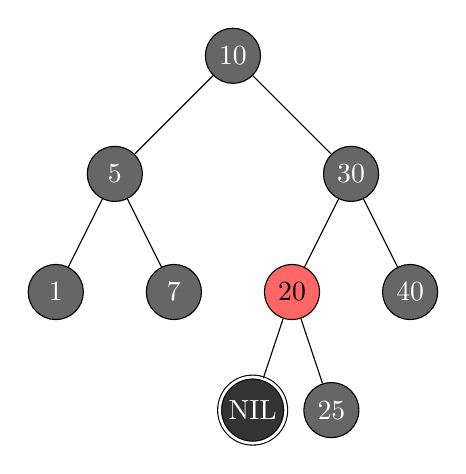
\begin{tikzpicture}[
  every node/.style={draw, circle, inner sep=2pt, minimum size=0.7cm},
  level/.style={sibling distance=3cm/#1, level distance=1.5cm},
  black/.style={fill=black!60, text=white},
  red/.style={fill=red!60},
  doubleblack/.style={fill=black!80, text=white, double=white, double distance=1pt}
]
\node[black] {10}
  child {node[black] {5}
    child{node[black] {1}} 
    child{node[black] {7}}
  }
  child {node[black] {30}
    child{node[red] {20}
        child{node[doubleblack] {NIL}}
        child{node[black]{25}}
    }
    child{node[black]{40}}
  };
\end{tikzpicture}
\end{center}
We see that this is the case in which sibling and both children are black, applying the rules we get,
\begin{center}
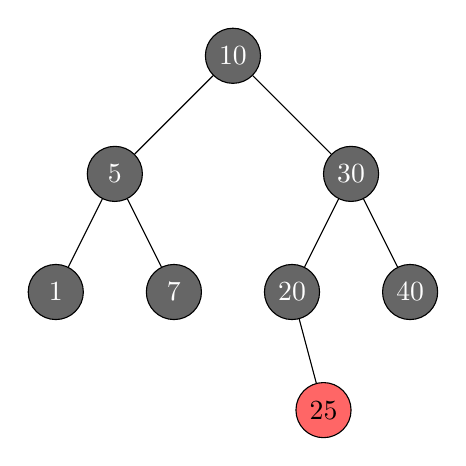
\begin{tikzpicture}[
  every node/.style={draw, circle, inner sep=2pt, minimum size=0.7cm},
  level/.style={sibling distance=3cm/#1, level distance=1.5cm},
  black/.style={fill=black!60, text=white},
  red/.style={fill=red!60},
  doubleblack/.style={fill=black!80, text=white, double=white, double distance=1pt}
]
\node[black] {10}
  child {node[black] {5}
    child{node[black] {1}} 
    child{node[black] {7}}
  }
  child {node[black] {30}
    child{node[black] {20}
        child{node[xshift=0.4cm][red]{25}}
    }
    child{node[black]{40}}
  };
\end{tikzpicture}
\end{center}

\subsection{Trivial Cases}
\subsubsection{DB is the root:}
Simply convert it into a single black node.

\subsubsection{If node to be deleted is \textcolor{red}{red}:}
Remove the node as it doesn't change the black height.
\pagebreak
\section{Pseudo code for Deletion and Deletion Fixup}
\begin{algorithm}[h]
    \caption{RB-Tree Deletion}
    \begin{algorithmic}[1]
    \Procedure{RB-Delete}{$T,z$}
    \State $y \gets z$
\State $y-original-color \gets y.color$
\If{$z.left = nil$}
\State $x \gets z.right$
\State \Call{RB-Transplant}{$T,z,z.right$}
\ElsIf{$z.right = nil$}
\State $x \gets z.left$
\State \Call{RB-Transplant}{$T,z,z.left$}
\Else
\State $y \gets$ \Call{Tree-Minimum}{$z.right$}
\State $y-original-color \gets y.color$
\State $x \gets y.right$
\If{$y.parent = z$}
\State $x.parent \gets y$
\Else
\State \Call{RB-Transplant}{$T,y,y.right$}
\State $y.right \gets z.right$
\State $y.right.parent \gets y$
\EndIf
\State \Call{RB-Transplant}{$T,z,y$}
\State $y.left \gets z.left$
\State $y.left.parent \gets y$
\State $y.color \gets z.color$
\EndIf
\If{$y-original-color = Black$}
\State \Call{RB-Delete-Fixup}{$T,x$}
\EndIf
    \EndProcedure
    \end{algorithmic}
\end{algorithm}

\begin{algorithm}[H]
    \caption{RB-Tree-Deletion-FixUp}
    \begin{algorithmic}[1]
        \Procedure{RB-DELETE-FIXUP}{$T,z$}
        \While{$x \neq T.root$ and $x.color = Black$}
        \If{$x = x.parent.left$}
        \State $w \gets x.parent.right$
        \If{$w.color = Red$}
        \State $w.color \gets Black$
        \State $x.parent.color \gets Red$
        \State \Call{Left-Rotate}{$T,x.parent$}
        \State $w \gets x.parent.right$
        \EndIf
        \If{$w.left.color = Black$ and $w.right.color = Black$}
        \State $w.color \gets Red$
        \State $x \gets x.parent$
        \Else
        \If{$w.right.color = Black$}
        \State $w.left.color \gets Black$
        \State $w.color \gets Red$
        \State \Call{Right-Rotate}{$T,w$}
        \State $w \gets x.parent.right$
        \EndIf
        \State $w.color \gets x.parent.color$
        \State $x.parent.color \gets Black$
        \State $w.right.color \gets Black$
        \State \Call{Left-Rotate}{$T,x.parent$}
        \State $x \gets T.root$
        \EndIf
        \Else
        \State $w \gets x.parent.left$
        \If{$w.color = Red$}
        \State $w.color \gets Black$
        \State $x.parent.color \gets Red$
        \State \Call{Right-Rotate}{$T,x.parent$}
        \State $w \gets x.parent.left$
        \EndIf
        \If{$w.right.color = Black$ and $w.left.color = Black$}
        \State $w.color \gets Red$
        \State $x \gets x.parent$
        \Else
        \If{$w.left.color = Black$}
        \State $w.right.color \gets Black$
        \State $w.color \gets Red$
        \State \Call{Right-Rotate}{$T,w$}
        \State $w \gets x.parent.left$
        \algstore{example-algo}
    \end{algorithmic}
\end{algorithm}

\begin{algorithm}
\caption{Contd.}
\begin{algorithmic}[1]
\algrestore{example-algo}
\EndIf
\State $w.color \gets x.parent.color$
\State $x.parent.color \gets Black$
\State $w.left.color \gets Black$
\State \Call{Right-Rotate}{$T,x.parent$}
\State $x \gets T.root$
\EndIf
\EndIf
\EndWhile
\State $x.color \gets Black$
\EndProcedure
\end{algorithmic}
\end{algorithm}

\section{RB Tree height proof}
\begin{proof}
We will prove by induction on the number of nodes $n$ in the tree that the maximum height of a red-black tree with $n$ nodes is at most $2 \log_2(n+1)$.

\textbf{Base Case:} When $n=1$, the tree consists of a single black root node, and its maximum height is 0. The inequality $0 \leq 2\log_2(1+1)$ holds, so the base case is true.

\textbf{Inductive Hypothesis:} Assume that for any red-black tree with $k$ nodes, where $1 \leq k \leq n$, the maximum height is at most $2 \log_2(k+1)$.

\textbf{Inductive Step:} Consider a red-black tree with $n+1$ nodes. Let $T$ denote the tree's root and $T_l$ and $T_r$ denote its left and right subtrees, respectively. Let $h_l$ and $h_r$ denote the maximum heights of $T_l$ and $T_r$, respectively.

Since $T$ is black and both of its children are red, the maximum height of $T$ is $1 + \max{h_l, h_r}$. By the inductive hypothesis, we have $h_l \leq 2\log_2(k_l+1)$ and $h_r \leq 2\log_2(k_r+1)$, where $k_l$ and $k_r$ denote the number of nodes in $T_l$ and $T_r$, respectively. Therefore,

\begin{align*}
 \text{max\_height}(T) &= 1 + \max{(h_l, h_r)} \\
 &\leq 1 + \max{(2\log_2(k_l+1), 2\log_2(k_r+1))} \\
 &= 1 + 2\lg\left[\max{((k_l+1), (k_r+1))}\right] \\
 &\leq 1 + 2\log_2(k_l + k_r + 2) \\
 &\leq 2\log_2(n+2) \\
 &= 2\log_2[(n+1)+1]
\end{align*}

Thus, the maximum height of a red-black tree with $n+1$ nodes is at most $2\log_2(n+2)$. By induction, the statement is true for all $n \geq 1$.
\end{proof}
\end{document}